\documentclass[11pt,letterpaper]{article}
\usepackage[margin=1in]{geometry}
\usepackage[T1]{fontenc}
\usepackage[utf8]{inputenc}
\usepackage{lmodern,microtype}
\usepackage{amsmath,amssymb,amsthm,mathtools}
\usepackage{graphicx,booktabs,longtable,tabularx,array}
\usepackage[dvipsnames]{xcolor}
\usepackage{enumitem,listings,needspace}
\usepackage[numbers,sort&compress]{natbib}
\usepackage[font=small,labelfont=bf]{caption}
\usepackage{fancyhdr,hyperref}
\hypersetup{colorlinks=true,linkcolor=MidnightBlue,citecolor=MidnightBlue,
 urlcolor=MidnightBlue,pdftitle={Certified Potts Filters and Order-Controlled Algebra for Unknot Recognition},
 pdfauthor={ProveIt research continuation}}
\urlstyle{same}
\setlength{\emergencystretch}{2em}
\setlength{\parskip}{0.25em}
\setlist{itemsep=0.25em,topsep=0.4em}
\pagestyle{fancy}
\fancyhf{}
\fancyhead[L]{\small ProveIt: unknot recognition}
\fancyhead[R]{\small Research continuation, 8 October 2026}
\fancyfoot[C]{\thepage}
\setlength{\headheight}{14pt}
\newtheorem{theorem}{Theorem}[section]
\newtheorem{proposition}[theorem]{Proposition}
\newtheorem{lemma}[theorem]{Lemma}
\newtheorem{corollary}[theorem]{Corollary}
\theoremstyle{definition}
\newtheorem{definition}[theorem]{Definition}
\newtheorem{question}[theorem]{Research question}
\theoremstyle{remark}
\newtheorem{remark}[theorem]{Remark}
\newcommand{\F}{\mathbb F}
\newcommand{\Z}{\mathbb Z}
\newcommand{\Q}{\mathbb Q}
\newcommand{\R}{\mathbb R}
\newcommand{\poly}{\operatorname{poly}}
\renewcommand{\wr}{\operatorname{wr}}
\newcommand{\tr}{\operatorname{tr}}
\newcommand{\im}{\operatorname{im}}
\newcommand{\rk}{\operatorname{rank}}
\newcommand{\End}{\operatorname{End}}
\newcommand{\Kh}{\operatorname{Kh}}
\newcommand{\fall}[2]{(#1)_{\underline{#2}}}
\newcommand{\pair}[2]{(#1,#2)}
\newcommand{\code}[1]{\texttt{\small #1}}
\newcommand{\claim}[1]{\par\smallskip\noindent\textbf{Status.} #1\par\smallskip}
\lstset{basicstyle=\ttfamily\footnotesize,columns=fullflexible,
 breaklines=true,frame=single,rulecolor=\color{black!20},
 backgroundcolor=\color{black!2},keepspaces=true,showstringspaces=false,
 xleftmargin=0.3em,xrightmargin=0.3em,aboveskip=0.8em,belowskip=0.8em}
\title{\LARGE\bfseries Certified Potts Filters and\\[0.3em]
Order-Controlled Algebra for\\[0.3em]Unknot Recognition\\[0.7em]
\large Exact arithmetic, component factorization, adversarial examples,\\
and a precise research program toward quasi-polynomial complexity}
\author{Research continuation for the ProveIt project}
\date{8 October 2026\\[0.3em]\small Baseline commit
\texttt{86f23490006c880cd01db9bec10761d39c6395c8}}
\begin{document}
\maketitle
\begin{abstract}
We develop and implement a certified scalar preprocessing improvement for
ProveIt's unknot recognizer. A signed checkerboard Potts transfer replaces
the current Jones filter's arbitrary matching frontier by equality patterns
of a fixed number of spin colors. For every crossing order of a connected
plane knot diagram, the number of active vertices of either Tait graph is
at most half the number of cut diagram edges. This yields
$\poly(n,w)q^{w/2}$ arithmetic work at fixed integer $q$, with all normalization
and coefficient lengths accounted for. Independent processed components
can be represented by separate tensors; a relative-color alignment formula
then gives a stronger bound in terms of the largest component frontier.

For $q\ge5$, computations take place exactly in
$\Z[x]/(x^2-(q-2)x+1)$, using integer pairs and no floating point.
An essential adversarial calculation shows that the previously studied
$q=5$ specialization is identically equal to the unknot value on an infinite
family of nontrivial weaving knots. Every exact $q\ge6$ specialization
detects every nontrivial knot in that family. This motivates $q=6$ for the
new exact backend without asserting that a single Jones value detects
all knots.

We also prove a residue characteristic-polynomial annihilator and sharp
radical-matrix nilpotence bounds over truncated polynomial rings. These
give short inverse and Fitting certificates for supplied same-matching
endomorphisms, extending the scope of earlier scalar splitting.
The package includes implementations, integration changes, independent
smoothing-cube and algebraic oracles, raw benchmark records, and reproducible
certificate replay. The Potts correspondence and single-exponential
width algorithms have substantial prior literature. Our contribution is
their precise, audited implementation and the associated scope analysis
for this repository. A complete quasi-polynomial unknot recognition bound
is not established.
\end{abstract}
\clearpage
\tableofcontents
\clearpage
\section{Outcome, scope, and the audited baseline}\label{sec:scope}

The immediate outcome is a new family of exact Jones obstruction backends,
together with a component factorization that improves their dependence on
the geometry of a supplied crossing order. These are useful pieces of a
complete recognizer. They are not, by themselves, complete recognition
algorithms: inequality with the unknot's Jones value proves knottedness,
whereas equality requires another method.

This distinction determines both the software interface and the mathematical
claims. In the implementation, a successful obstruction returns
\code{KNOTTED}. Equality returns an inconclusive result. Exhausting a local
filter budget also returns an inconclusive result, with its reason recorded;
it does not produce a topological verdict. The enclosing recognizer retains
its existing complete Khovanov fallback, subject to the user's global resource
limits. Thus a bounded execution can still return \code{UNKNOWN}.

\subsection{What was inspected and preserved}

The baseline is ProveIt commit
\code{86f23490006c880cd01db9bec10761d39c6395c8}, dated
8 October 2026 \cite{proveit2026}. The source snapshot includes the Python
\code{fastunknot} package, its fixtures and tests, the synthesis sources, and
the report summaries. Downloaded source blobs were checked against their
Git object identifiers. The included reference implementation is immutable
within the experiment package. The baseline test suite passed all 134 tests.

The baseline already contains substantial work: short-braid certificates,
Seifert and descending-diagram tests, Reidemeister simplification,
connected-sum handling, modular Alexander and Jones obstructions,
optional exact Alexander computation, and several exact Khovanov scanner
representations. Earlier research also introduced canonical multiplicities,
shared morphisms, radical perturbation inverses, saturated or Euler-assisted
terminal decisions, homological windows, and scalar Fitting decompositions
\cite{report07,report08,report09,report10,report11,report12}.
Those ideas remain predecessors, rather than contributions claimed here.
The immediately preceding continuation's scalar splitting and
common-nilpotent decision shortening were inspected separately; the
ring-valued extension in Section~\ref{sec:residue} is carefully distinguished
from them.

The current Jones filter stores boundary smoothing matchings and their
scalar coefficients. For an arbitrary cut with $w$ endpoints, a universal
matching count is $(w-1)!!$, not a Catalan number. A Catalan bound requires
additional boundary-order geometry that an arbitrary crossing prefix need
not possess. This creates an opportunity to change the scalar representation
without making an invalid noncrossing assumption.

\subsection{Claims and their evidential status}

\begingroup\small
\begin{longtable}{@{}>{\raggedright\arraybackslash}p{0.28\textwidth}p{0.67\textwidth}@{}}
\toprule
Claim & Status and limit\\
\midrule
\endfirsthead
\toprule Claim & Status and limit\\ \midrule
\endhead
Signed Tait/Potts expression for Jones values &
Classical; derived in the repository's normalization and checked against an
independent smoothing cube.\\
At most $w/2$ active Tait vertices &
Proved here by a direct boundary-transition count for every crossing order
of a connected plane knot shadow.\\
Fixed-$q$ equality-pattern transfer &
Implemented and verified; costs $\poly(n,w)q^{w/2}$, with linear-in-$n$
coefficient bit lengths for fixed $q$.\\
Independent-component transfer &
Implemented; a relative-color merge restores precisely the information
needed when components first interact.\\
$q=5$ blind weaving family &
Proved by specializing the classical three-braid trace formula; preserved as
an adversarial regression family.\\
$q\ge6$ detects that family &
Proved; says nothing universal about other knot families.\\
Residue-polynomial Fitting certificates &
Proved for matrices over specified commutative truncated rings; verified by
a separate algebraic oracle.\\
Quasi-polynomial full recognition &
Conditional research goal. No complete complexity proof or complete
quasi-polynomial implementation is supplied.\\
\bottomrule
\caption{The claim ledger. A proof supplied in this article is not a claim
of literature-wide priority.}
\label{tab:claims}\\
\end{longtable}
\endgroup

\subsection{Prior literature and the nature of the improvement}

The Potts formulation of the Jones polynomial belongs to the classical
state-model literature \cite{kauffman1987,sokal2005,moffatt2011}.
Meichanetzidis and Kourtis explicitly used the same integer-color
specializations, including $q=5$, in tensor-network evaluation
\cite{meichanetzidis2019}. Makowsky established bounded-treewidth
tractability for signed Tutte and Kauffman computations
\cite{makowsky2005}. Maria gave single-exponential width dependence for
general quantum link invariants \cite{maria2021}. The broad statement
that Jones evaluation is single exponential in a suitable width is therefore
not a new result.

The contribution appropriate to this continuation is more concrete. We
derive a bound directly in the crossing-order parameter used by ProveIt,
make equality-pattern aggregation and normalization explicit, implement exact
quadratic arithmetic, retain resource-safe recognition semantics, identify a
structural failure of the $q=5$ point, and supply measurements including
regressions. The component factorization and residue-algebra sections give
additional, independently checkable improvements whose exact applicability
is stated.

The public \code{openai/math} collection was inspected as suggested by the
user \cite{openaimath2026}. It did not supply a missing unknot-recognition
theorem. Its useful role here is methodological: formulate explicit lemmas,
test a proposed general claim on adversarial families, and preserve enough
artifacts that independent readers can reproduce the calculation. None of
the results in this article is attributed to that collection without a
specific mathematical dependency.

\subsection{Complexity terminology}

Throughout, $n$ is the number of crossings in the supplied diagram, $w$ is a
maximum cut-edge count for a crossing order, and $q$ is an integer color
count. A statement for fixed $q$ does not hide a growing input parameter.
We use \emph{quasi-polynomial} in the broad sense
$\exp((\log(n+2))^{O(1)})$, and state the stronger bound
$n^{O(\log n)}$ explicitly when it is obtained. Arithmetic-operation bounds
and bit-operation bounds are separated. Timing improvements on a finite
corpus are not asymptotic evidence by themselves.

\section{The signed Tait partition function in the repository convention}
\label{sec:potts}

\subsection{Input, embedding, and signs}

Let $D$ be a classical one-component knot diagram with $n>0$ crossings.
Its shadow is a connected plane four-valent multigraph. The public input
validator checks that the supplied planar-diagram code has the required
edge incidences, one link component, and spherical rotation system.
The following construction uses that embedding, not an abstract graph
with its rotation data discarded.

Choose one checkerboard color. The Tait graph $G=(V,E)$ has one vertex for
each region of that color and one edge for each crossing. It can contain
loops and parallel edges. Write $v=|V|$. At a crossing $e$, designate as the
\emph{omitted} smoothing the one that leaves the two selected-color
corners disconnected across that crossing. Its bracket coefficient is
$A^{\epsilon_e}$, where $\epsilon_e\in\{1,-1\}$.
The included smoothing has coefficient $A^{-\epsilon_e}$.
This convention, which is checked from the local darts in the implementation,
avoids assuming that an alternating-diagram sign rule applies to all
diagrams. Put
\[
 s=\sum_{e\in E}\epsilon_e,\qquad \delta=-A^2-A^{-2}.
\]
We use the \emph{full} bracket $B_D(A)$, for which an isolated circle has
value $\delta$. The normalized Jones polynomial is
\begin{equation}
 V_D(A^{-4})=\frac{B_D(A)}{\delta(-A^3)^{\wr(D)}}.
 \label{eq:jones-normalization}
\end{equation}
Consequently the full bracket of an unknot diagram with writhe $\wr(D)$ is
$\delta(-A^3)^{\wr(D)}$. Losing the initial circle factor would invalidate the
obstruction.

\begin{lemma}[State circles]\label{lem:circles}
For $S\subseteq E$, let $k(S)$ be the number of components of the spanning
subgraph $(V,S)$, including isolated vertices. The associated smoothing state
has $c(S)=2k(S)-v+|S|$ circles.
\end{lemma}
\begin{proof}
A regular neighborhood of $(V,S)$ in the sphere retracts to that subgraph,
so its Euler characteristic is $v-|S|$. Its $k(S)$ components are planar
surfaces. If their total number of boundary components is $c$, their Euler
characteristic is $2k(S)-c$. Those boundary components are the smoothing
circles. Equating the two expressions proves the formula. An isolated vertex
has a disk neighborhood and contributes one circle, as required. Loops and
parallel edges are included in the same argument.
\end{proof}

\subsection{From smoothing states to spins}

The multivariate random-cluster partition function is
\[
 Z_G(Q,\{z_e\})=\sum_{S\subseteq E}Q^{k(S)}\prod_{e\in S}z_e.
\]
At a positive integer $Q=q$, the Fortuin--Kasteleyn identity is
\begin{equation}
 Z_G(q,\{z_e\})
 =\sum_{\sigma:V\to[q]}
   \prod_{e=uv}\bigl(1+z_e[\sigma(u)=\sigma(v)]\bigr).
 \label{eq:fk}
\end{equation}
To verify it, expand the product on the right. For each selected subset
$S$, the spin assignment must be constant on each component of $(V,S)$,
giving exactly $q^{k(S)}$ choices. This also proves the identity for loops,
parallel edges and isolated vertices \cite{sokal2005}.

\begin{proposition}[Signed partition-function formula]\label{prop:potts}
In the rational-function field, or after localizing at $\delta$, with
$Q=\delta^2$ and $z_e=\delta A^{-2\epsilon_e}$,
\begin{equation}
 B_D(A)=\delta^{-v}A^s Z_G(Q,\{z_e\}).
 \label{eq:full-bracket}
\end{equation}
\end{proposition}
\begin{proof}
The smoothing indexed by $S$ contributes
\[
 A^s\prod_{e\in S}A^{-2\epsilon_e}\,
 \delta^{2k(S)-v+|S|}.
\]
Factor out $\delta^{-v}A^s$ and sum. The remaining term for $S$ is
$(\delta^2)^{k(S)}\prod_{e\in S}(\delta A^{-2\epsilon_e})$.
\end{proof}

Set $x=A^4$. Then
\[
 Q=x+2+x^{-1},\qquad z_e=-1-x^{-\epsilon_e}.
\]
Thus the spin interaction has the especially simple form
\begin{equation}
 h_e(a,b)=
 \begin{cases}
  -x^{-\epsilon_e},&a=b,\\
  1,&a\ne b.
 \end{cases}
 \label{eq:interaction}
\end{equation}
This is the signed interaction used in the earlier tensor-network
formulation \cite{meichanetzidis2019}. It allows all crossings to be processed
as local equality tests, without tracking smoothing connectivity.

\subsection{Eliminating fourth roots from normalization}

Since $\delta=-(x+1)A^{-2}$, substituting
\eqref{eq:full-bracket} into \eqref{eq:jones-normalization} gives
\begin{equation}
 V_D(A^{-4})
 =(-1)^{\wr(D)+v+1}A^E
   \frac{Z_G}{(x+1)^{v+1}},
 \qquad E=s-3\wr(D)+2(v+1).
 \label{eq:normalize-E}
\end{equation}

\begin{lemma}[Integral normalization exponent]\label{lem:parity}
For a knot, $E$ is divisible by four.
\end{lemma}
\begin{proof}
For a smoothing state with coefficient exponent $s_\sigma$ and circle
count $c_\sigma$, the residue
\[
 s_\sigma-3\wr(D)+2(c_\sigma-1)\pmod4
\]
is unchanged when one smoothing is flipped: the exponent changes by
$\pm2$ and the circle count by $\pm1$. In the oriented Seifert state,
$s_\sigma=\wr(D)$. The genus formula for a one-component Seifert surface
gives $c_\sigma-1\equiv n\equiv\wr(D)\pmod2$, so the residue is zero.
In the all-omitted state, $s_\sigma=s$ and $c_\sigma=v$.
Its expression differs from $E$ by four.
\end{proof}

Writing $h=E/4$, the exact equality test can therefore be performed as
\begin{equation}
 Z_G\stackrel{?}{=}Z_U,\qquad
 Z_U=(-1)^{\wr(D)+v+1}x^{-h}(x+1)^{v+1}.
 \label{eq:unknot-partition}
\end{equation}
No fourth root of $x$ is needed. This is an equality of algebraic integers in
the ring introduced in Section~\ref{sec:exact}. The comparison is obtained by
multiplying through the nonzero normalization factor; the implementation
never needs to divide by $x+1$.

The empty crossing diagram is handled separately as a single circle, with
$Z_G=Z_U=q$. For a link with $\ell$ components the parity residue in the lemma
would instead be $2(\ell-1)\pmod4$. This article and the public recognizer
require a knot; accepting all links without revisiting normalization would
be an unsupported generalization.

\section{Arbitrary crossing orders and equality-pattern states}
\label{sec:frontiers}

\subsection{A local half-frontier theorem}

Fix a permutation of the $n$ crossings, and let $P_i$ be its first $i$
crossings. Define $w_i$ to be the number of diagram edges with one endpoint
in $P_i$ and the other outside $P_i$. A loop at one crossing is never counted.
The scan width is $w=\max_i w_i$.

In the selected Tait graph, let $f_i$ be the number of vertices incident with
both a processed and an unprocessed Tait edge. These are precisely the spin
variables that must survive after step $i$. A vertex is introduced at its
first incident edge and forgotten after its last.

\begin{theorem}[Half-frontier bound]\label{thm:half}
For every crossing order of a connected plane knot shadow and either fixed
checkerboard color, $2f_i\le w_i$ for every $i$.
\end{theorem}
\begin{proof}
The boundary of each face of a connected plane graph is a single cyclic
dart walk. This remains true when a boundary repeats vertices or edges.
On the walk around a selected-color region, mark each crossing incidence
according as that crossing belongs to $P_i$ or its complement.
An active Tait vertex corresponds to a walk containing both marks.
A cyclic binary word with both symbols has at least two transitions.

Each transition traverses a shadow edge with endpoints of opposite status.
Conversely each such cut edge occurs on exactly one selected-color face
boundary. Count the transitions over all active selected-color regions.
There are at least $2f_i$ of them and at most $w_i$. This proves the claim.
\end{proof}

The result does not assume that the processed diagram is a disk tangle.
Repeated face incidences, Tait loops, parallel edges and articulation points
do not invalidate the proof. Connectedness matters: a face of a disconnected
plane graph can have several boundary walks, each monochromatic in status,
while their union contains both statuses. The one-knot input condition
avoids that case. Classical relations between a plane graph and its medial
graph provide broader width context \cite{seymour1994}; the direct proof
above supplies the exact inequality used by this implementation.

Both checkerboard colors satisfy the theorem. The code computes their
profiles and chooses a single color minimizing the pair
$(\max_i f_i,\sum_i f_i)$, with a deterministic tie break.
It does not switch colors at individual steps. A pointwise minimum of two
profiles would require a tensor conversion that has not been constructed.

\subsection{Quotienting names of colors}

The Potts interaction depends only on equality of spins. The symmetric group
$S_q$ acts on every spin assignment by relabeling colors and preserves every
weight. On an ordered active set of $f$ vertices, an orbit is a set partition
into at most $q$ blocks. Encode it by its restricted-growth word, for example
$0102$ for a pattern whose first and third vertices have equal spins and
whose other two spins are distinct from those and from each other.

Let
\begin{equation}
 B_q(f)=\sum_{k=0}^{\min(q,f)}
             \left\{\begin{matrix}f\\k\end{matrix}\right\}
 \le q^f,\qquad B_q(0)=1.
 \label{eq:orbitcount}
\end{equation}
For fixed $q$ and large $f$, $B_q(f)\sim q^f/q!$.
These are partitions by \emph{color equality}, not partitions by graph
connectivity and not planar noncrossing partitions.

\begin{definition}[Aggregate coefficient]
The coefficient of an equality pattern is the sum of the partial Potts
weights over all labeled spin assignments on the introduced vertices whose
restriction to the active set has that pattern. Spins on forgotten vertices
have already been summed out.
\end{definition}
The word \emph{sum} is essential. A per-representative value and an
orbit-aggregate value obey different introduction rules.

\begin{proposition}[Exact transfer rules]\label{prop:orbit}
The following operations maintain the aggregate-coefficient invariant over
any commutative coefficient ring with a specified unit $x$.
\begin{enumerate}
\item To introduce a vertex when $k$ color classes are active, create one
extension for each existing class with multiplier $1$, and, if $k<q$, one
new-class extension with multiplier $q-k$.
\item To process an edge, multiply by $-x^{-\epsilon_e}$ if its endpoint
classes agree and by $1$ otherwise.
\item To forget vertices, delete their positions, canonically relabel the
remaining word, and add coefficients with the same resulting word.
\end{enumerate}
\end{proposition}
\begin{proof}
For each labeled active assignment, a new spin has exactly one choice for
each currently used color and $q-k$ choices among unused colors. This proves
the first rule. The edge weight is constant on an equality orbit, proving
the second. The last rule is the pushforward of a finite sum under restriction
to a smaller active set. Once a vertex is forgotten, no future edge is
incident with it, so its color name imposes no further condition.
\end{proof}

At a crossing at most two Tait vertices are introduced. The implementation
combines introduction, multiplication and forgetting, inserting results
directly into the following table. It records transient insertions as well
as completed tables when reporting its maximum state count. A scalar
coefficient that is exactly zero is removed. Cancellation changes actual
state counts but is not used to justify the worst-case bound.

\begin{theorem}[Fixed-color transfer complexity]\label{thm:transfer}
For a supplied crossing order of width $w$ and fixed integer $q$, the
one-tensor Potts transfer computes the partition function in
\[
 n\,\poly(w,\log n)\,q^{\lfloor w/2\rfloor+2}
\]
coefficient-ring operations and key-management work, and uses
$\poly(w,\log n)q^{\lfloor w/2\rfloor}$ coefficient slots and key storage.
Preparation also uses $O(n)$ storage; coefficient bit memory is treated
separately below. This replaces the general factorial state-count envelope
by a single-exponential upper bound, without asserting that the baseline
always realizes its larger envelope.
\end{theorem}
\begin{proof}
After a step there are at most $B_q(f_i)\le q^{w/2}$ keys.
Introducing at most two vertices has at most $q^2$ labeled choices per
state; orbit aggregation cannot increase that count. Edge multiplication
and forgetting use polynomial work in the key length. Sum over $n$ edges.
Two successive tables and a bounded extension list suffice.
A deterministic comparison-based dictionary adds a polynomial factor in
$w$ and $\log n$; it does not change the exponential term.
\end{proof}

The actual Python implementation uses dictionaries. Its timings concern
that implementation, while the deterministic bound above can be realized
with balanced search structures or sorted merging. Order construction is
separate: the repository's heuristic is polynomial work and is timed
explicitly in end-to-end measurements. No optimal-width order is assumed
to be available for free.

\begin{corollary}\label{cor:widthclasses}
For fixed $q$, the scalar filter is polynomial time on supplied orders with
$w=O(\log n)$ and runs in $n^{O(\log n)}$ time on supplied orders with
$w=O((\log n)^2)$, including the bit costs of Section~\ref{sec:exact}.
\end{corollary}
The preceding matching count gives $2^{O(w\log w)}$ as a general envelope.
At $w=O((\log n)^2)$ that is still quasi-polynomial in the broad definition,
but contains an additional $\log\log n$ in the exponent.
The sharper Potts bound should not be described as having changed a
non-quasi-polynomial class into a quasi-polynomial one at that same width.

\section{Division-free quadratic arithmetic and bit complexity}
\label{sec:exact}

\subsection{An exact ring for each integer color count}

Fix an integer $q\ge5$ and put
\[
 R_q=\Z[x]/(x^2-(q-2)x+1).
\]
The discriminant $(q-2)^2-4$ lies strictly between the consecutive squares
$(q-3)^2$ and $(q-2)^2$, so the polynomial is irreducible over $\Q$.
In either real embedding,
\[
 x+x^{-1}=q-2,\qquad x^{-1}=q-2-x,\qquad (x+1)^2=qx.
\]
In particular $x$ is a unit. Each element has a unique representation
$a+bx$ with $a,b\in\Z$. Pair inequality is exact inequality of the algebraic
numbers; it is not a numerical tolerance test.

For $q=6$, the positive roots are $2+\sqrt3$ and $2-\sqrt3$.
The Jones variable in our derivation is $t=A^{-4}=x^{-1}$.
Changing embeddings interchanges these reciprocal values; equality to $1$
is preserved because the coefficients are rational integers.
The code works in the ring and need not select a real embedding.

\begin{table}[htbp]
\centering\small
\begin{tabular}{@{}ll@{}}
\toprule
Operation & Pair formula\\
\midrule
Addition & $(a,b)+(c,d)=(a+c,b+d)$\\
Multiplication & $(a,b)(c,d)=(ac-bd,\ ad+bc+(q-2)bd)$\\
Multiply by $-x$ & $(a,b)\mapsto(b,\ -a-(q-2)b)$\\
Multiply by $-x^{-1}$ & $(a,b)\mapsto(-(q-2)a-b,\ a)$\\
Inverse of $x$ & $x^{-1}=(q-2,-1)$\\
\bottomrule
\end{tabular}
\caption{Exact arithmetic used by the transfer. Full pair multiplication
is needed for normalization and component merges; a single-edge transfer
uses only additions and small integer multiples.}
\label{tab:pairs}
\end{table}

Equations~\eqref{eq:interaction} and \eqref{eq:unknot-partition} now define a
division-free one-tensor algorithm. Negative powers in normalization are
powers of the explicit unit $x^{-1}$. Fast powering is exact. No prime choice,
probability-of-error estimate, or floating-point precision policy is required.

\begin{proposition}[Sound exact obstruction]\label{prop:obstruction}
If the partition function and $Z_U$ are unequal as pairs in $R_q$, then
$D$ is a nontrivial knot. If they are equal, the computation gives no
unknot certificate.
\end{proposition}
\begin{proof}
The nonzero normalization factor in \eqref{eq:normalize-E} identifies
partition equality with equality of the selected normalized Jones value to
$1$. Every unknot has normalized Jones polynomial $1$, so inequality rules
it out. The converse would require an additional detection theorem that
is not available here. Section~\ref{sec:blind} gives explicit failures at
$q=5$.
\end{proof}

\subsection{Coefficient lengths}

Let $\|a+bx\|_1=|a|+|b|$. The two equal-spin multiplication maps in
Table~\ref{tab:pairs} have induced $\ell^1$ norm at most $q-1$.

\begin{theorem}[Linear coefficient bit lengths]\label{thm:bits}
After $i$ edges and $I$ introduced vertices, every aggregate table
coefficient, including every partial sum inserted into the next table,
satisfies
\[
 \|a+bx\|_1\le q^I(q-1)^i\le q^v(q-1)^n.
\]
Its magnitude coefficients therefore have at most
\[
 \left\lfloor v\log_2q+n\log_2(q-1)\right\rfloor+1
\]
bits. For fixed $q$ this is $O(n)$, and for $q=6$ the simpler upper bound
$5n+4$ is valid.
\end{theorem}
\begin{proof}
Every labeled assignment of the introduced vertices contributes a product
of $i$ edge weights. Its norm is at most $(q-1)^i$.
An aggregate coefficient is a sum over a subset of at most $q^I$
assignments, so the triangle inequality proves the first bound. Partial
insertions are sums over subsets of the same histories and obey the same
bound. The connected Tait graph has $v\le n+1$, giving the stated bit length.
For $q=6$, $\log_2 6+\log_2 5=\log_2 30<5$ and
$\log_2 6<3$, proving the convenient integer bound.
\end{proof}

The normalization pair is also polynomial in bit length:
\[
 \|Z_U\|_1\le(q-1)^{|h|}q^{v+1},\qquad
 |h|\le n+(v+1)/2.
\]
Thus no hidden exponential coefficient size invalidates the transfer's
width bound. At fixed $q$, a single-edge update costs $O(n)$ elementary bit
operations apart from key management. Ordinary multiplication of
$O(n)$-bit integers suffices for powering and component merges; faster
integer multiplication can be used without changing the width dependence.

The coefficient-length bound is a worst-case upper bound, not an assertion
that every table entry reaches it. The experiment record reports the
largest coefficient actually inserted. It does not treat Python object
overhead as coefficient bits, and neither number is a process-memory limit.

\subsection{The modular comparison backend}

For a second implementation path the package includes a modular $q=5$
backend over $p=2^{61}-1$, with a root of $x^2-3x+1$ and a compatible fourth
root $A$. It compares the full bracket at precisely that $A$ with
$\delta(-A^3)^{\wr(D)}$. The constants are checked algebraically on import.
The old matching transfer can be evaluated at the same $A$, making an
apples-to-apples scalar comparison possible.

A modular mismatch is also a sound obstruction. A modular match may arise
from reduction modulo $p$ or from a genuine specialization collision.
Increasing the number of primes can address the former but cannot repair
the latter. In particular it cannot repair the family in
Section~\ref{sec:blind}. The exact backend makes this distinction observable.

\section{Factoring intermediate components instead of correlating all spins}
\label{sec:factorization}

\subsection{Why the global orbit table can still be wasteful}

A poor crossing order can create several disjoint components of processed
Tait edges. Before any processed edge joins them, their partial weights
factor. A global $S_q$ orbit table nevertheless records whether an active
spin in one component happens to have the same color as a spin in another.
Those relative color identities matter only when a future edge first
connects the two components. Recording them earlier can create many keys
with an exactly factorizable coefficient.

This is an exact independence statement about the processed interaction
graph. It does not follow merely because two groups of vertices appear far
apart in a drawing, nor does it assume a graph separator whose crossing
interactions have been discarded. We keep one tensor for each connected
component of the graph formed by introduced vertices and processed edges.
Connectivity through a forgotten vertex remains connectivity: forgetting
does not undo an interaction already summed into the tensor.

An isolated newly introduced vertex has the one-key table
$\{(0)\mapsto q\}$. An edge internal to a component uses the usual equality
weight and forgetting operation. When no active vertices remain in a
component, its scalar partition factor is multiplied into the accumulated
scalar and its tensor is released. Only an edge joining two distinct
processed components requires a new operation.

\subsection{The relative-color merge}

Let a left pattern have $k$ classes and a right pattern have $\ell$ classes.
Within each pattern, distinct classes must receive distinct colors.
Across the two patterns, an arbitrary partial bijection may identify
some left and right classes. If $j$ pairs are identified, the merged pattern
has $K=k+\ell-j$ classes, and it is possible exactly when $K\le q$.
The number of such alignments is
\begin{equation}
 A_q(k,\ell)=
 \sum_{\substack{0\le j\le\min(k,\ell)\\k+\ell-j\le q}}
 \binom{k}{j}\binom{\ell}{j}j!.
 \label{eq:alignments}
\end{equation}
It is at most $q!$ when $k,\ell\le q$. One way to see this bound is to fix
distinct actual colors on all left classes and inject the alignment choices
into the injective assignments of colors to the $\ell$ right classes by
assigning fresh colors in a prescribed order. There are
$\fall{q}{\ell}\le q!$ such assignments. The implementation enumerates
alignments directly, giving fresh classes their next canonical label.

\begin{theorem}[Aggregate component merge]\label{thm:merge}
Work over $R_q$, or over a field of characteristic zero or greater than $q$.
Suppose the left and right orbit coefficients are $C_L$ and $C_R$.
For one relative alignment with $K$ total classes, its aggregate coefficient
before the joining edge is applied is
\begin{equation}
 \frac{C_L}{\fall{q}{k}}\,
 \frac{C_R}{\fall{q}{\ell}}\,
 \fall{q}{K}.
 \label{eq:merge}
\end{equation}
After multiplication by the joining-edge weight, ordinary forgetting
and canonical aggregation produce the correct merged tensor.
\end{theorem}
\begin{proof}
The orbit of a pattern with $k$ nonempty classes has
$\fall{q}{k}$ labeled active assignments. Color relabeling preserves the
sum over forgotten spins, so all those active assignments have the same
partial value. That value is $C_L/\fall{q}{k}$. The same statement holds
on the right.

Before the joining edge, the two processed components share no vertex or
processed interaction, so their per-assignment partial values multiply.
The aligned combined pattern has $\fall{q}{K}$ labeled assignments.
Multiplying by this orbit size gives \eqref{eq:merge}.
Every combined pattern determines exactly its restrictions and its
partial-bijection alignment, so no term is omitted or counted twice.
The joining edge and restriction to surviving vertices then obey
Proposition~\ref{prop:orbit}.
\end{proof}

In the modular backend, $q<p$ makes every falling factorial a unit in
$\F_p$, and inverses can be precomputed. In the exact backend, each
coefficient is an integral multiple of its orbit size in $R_q$.
Both integer coordinates are therefore divisible by that positive integer.
The implementation checks the remainders and performs exact integer
division. It then multiplies the resulting pairs.
This operation uses no fraction field and no approximate division.
Unlike the one-tensor transfer, it is not literally division-free; the
divisions are certified divisions by known small integers at fixed $q$.

\subsection{A stronger parameter: the largest processed component}

For each step, consider each still-active processed component and count its
active vertices. Define $g$ to be the largest such count over all components
and all \emph{post-edge} steps. Thus $g\le\max_i f_i\le w/2$.

\begin{theorem}[Component-frontier complexity]\label{thm:componentwidth}
At fixed $q$, the factored transfer uses
\[
 n\,\poly(g,\log n)\,q!\,q^{g+2}
\]
coefficient operations and key-management work, with
$O(nq^g)$ logical table keys. Over $R_q$, coefficient bit lengths remain
$O(n\log q)$; the bit-operation bound is obtained by multiplying the
displayed work by a polynomial in $n\log q$.
\end{theorem}
\begin{proof}
An edge can cause only its two incident vertices to be forgotten: any
vertex whose last incident edge is the current edge must be an endpoint.
Therefore a component's pre-forget active set at this step has at most
$g+2$ vertices. For a merge, this set is the union of the two input active
sets, including newly introduced endpoints. If their sizes are $a,b$, then
$a+b\le g+2$. The number of pairs of input keys is at most
$q^a q^b\le q^{g+2}$; each pair has at most $q!$ alignments.
An internal edge has the same bound without the alignment factor.
There are $n$ edges and at most $O(n)$ active components.

For the exact coefficient bound, each component coefficient is a sum over
assignments on a subset of vertices and a product over its processed edges.
The argument of Theorem~\ref{thm:bits} applies componentwise. During a merge,
the division removes an orbit multiplicity, and the final insertion is a
sum over a subset of assignments on the union. Its length is again bounded
by the same global $q^v(q-1)^n$ envelope.
\end{proof}

Bounding each input component separately by $g$ and then multiplying two
$q^g$ tables would give the weaker exponent $2g$.
The fact that only the current edge's endpoints can be forgotten is what
gives the stronger $g+2$ bound. A measurement of the largest table size alone
would not prove either complexity result: merge Cartesian products and
alignment work must be counted.

\subsection{Implementation and remaining limitations}

The package supplies modular and exact factored kernels. Their state budget
bounds the sum of represented keys over current component tables. During an
update, the old input tables and their replacement may coexist; normalized
merge lists and cached alignment patterns also occupy memory.
Consequently that counter is a logical state budget, not an allocation or
resident-memory ceiling. Transition counts include each relative alignment
that is actually processed.

At $q=5$ there are at most $120$ alignments per input-key pair; at $q=6$
there are at most $720$. These constants can make factorization slower when
components repeatedly merge without having saved many keys. The measured
negative controls in Section~\ref{sec:experiments} are therefore essential.
The implementation does not factor a connected tensor merely because its
coefficient array happens to have low rank, and it does not split components
again when active graph connectivity changes. Such extensions require
additional algebra and are research topics rather than current guarantees.

\section{An infinite exact failure at five colors and its six-color repair}
\label{sec:blind}

\subsection{The weaving family as an adversarial test}

Let
\[
 W_m=\widehat{(\sigma_1\sigma_2^{-1})^m}.
\]
The strand permutation is a power of a three-cycle, so $W_m$ is a knot
exactly when $\gcd(m,3)=1$. Its displayed diagram has $2m$ crossings and
writhe zero. A familiar three-braid identity expresses its Jones polynomial
using reduced Burau matrices \cite{birman1985,alsukaiti2024}:
\begin{equation}
 V_{W_m}(t)=t+t^{-1}+\tr(M(t)^m),\qquad
 M(t)=
 \begin{pmatrix}
  1-t&-t^{-1}\\
  1&-t^{-1}
 \end{pmatrix}.
 \label{eq:weaving-jones}
\end{equation}
Direct calculation gives
\[
 \det M(t)=1,\qquad \tr M(t)=1-t-t^{-1}.
\]
Thus $T_m=\tr(M(t)^m)$ obeys
\[
 T_0=2,\quad T_1=1-t-t^{-1},\quad
 T_{m+1}=(1-t-t^{-1})T_m-T_{m-1}.
\]
Only this elementary recurrence is needed for the specialization audit.

\begin{theorem}[An exact five-color blind family]\label{thm:blind}
At either root of $t^2-3t+1=0$,
\[
 V_{W_m}(t)=3+2(-1)^m.
\]
In particular every odd $m\ge5$ with $3\nmid m$ gives a nontrivial knot
whose exact five-color Jones value equals the unknot value.
\end{theorem}
\begin{proof}
At this specialization, $t+t^{-1}=3$ and $\tr M=-2$.
The trace recurrence has solution $T_m=2(-1)^m$.
Equation~\eqref{eq:weaving-jones} gives the displayed value.
Nontriviality follows either from Theorem~\ref{thm:six} below or from
the determinant formula
\[
 \det(W_m)=L_{2m}-2
   =\left(\frac{3+\sqrt5}{2}\right)^m
    +\left(\frac{3-\sqrt5}{2}\right)^m-2>1
\]
for $m\ge2$ \cite{alsukaiti2024}. Here $L_j$ denotes the Lucas sequence.
For example $W_5$ has determinant $121$.
\end{proof}

This is a collision in a characteristic-zero number field. Both embeddings
have the same value, and every finite-field image in which the specialization
is defined inherits the equality. More precision, a conjugate root, or more
primes at the same $q=5$ point cannot solve it.
The statement is a direct consequence of a classical trace identity; we
make no claim that this particular consequence has not appeared elsewhere.
Its role here is to disprove an overly optimistic completeness inference and
to supply an infinite regression family.

\subsection{Why six colors changes this family}

\begin{theorem}[Every exact $q\ge6$ detects the nontrivial weaving members]
\label{thm:six}
Let $q\ge6$ be an integer and let $t+t^{-1}=q-2$.
For every $m\ge2$ such that $W_m$ is a knot,
$V_{W_m}(t)\ne1$.
\end{theorem}
\begin{proof}
Put $a=q-3\ge3$ and define
\[
 U_0=2,\qquad U_1=a,\qquad U_{m+1}=aU_m-U_{m-1}.
\]
The trace recurrence gives $T_m=(-1)^mU_m$, hence
\begin{equation}
 V_{W_m}(t)=a+1+(-1)^mU_m.
 \label{eq:qweaving}
\end{equation}
We have $U_2=a^2-2>a$. If $U_m>U_{m-1}>0$, then
$U_{m+1}>(a-1)U_m\ge2U_m$. Thus $U_m$ is positive and strictly
increasing for $m\ge1$.
For even $m\ge2$, \eqref{eq:qweaving} is greater than $1$.
For odd $m\ge3$, $U_m>a$ and the expression is less than $1$.
The remaining member $W_1$ has value $1$ and is the unknot.
\end{proof}

At $q=6$, the recurrence starts $2,3,7,18,47,123,\ldots$.
Thus $V_{W_5}=4-123=-119$ and $V_{W_7}=4-843=-839$.
These integer values in a quadratic specialization provide especially simple
independent checks of normalization and color count.

\begin{table}[htbp]
\centering
\begin{tabular}{@{}rrrrr@{}}
\toprule
$m$ & Crossings & Knot? & Exact $q=5$ value & Exact $q=6$ value\\
\midrule
1&2&yes&1&1\\
2&4&yes&5&11\\
4&8&yes&5&51\\
5&10&yes&1&$-119$\\
7&14&yes&1&$-839$\\
8&16&yes&5&2211\\
\bottomrule
\end{tabular}
\caption{Weaving specialization values, computed from the displayed trace
recurrence and independently checked by the transfer routines.}
\label{tab:weaving}
\end{table}

The equality-pattern spaces for $q=5$ and $q=6$ are identical for $f\le5$.
At $f=6$ their sizes are $202$ and $203$, respectively. On small frontiers,
changing the specialization can therefore improve detection with little
change in represented state count. Its worst-case exponential base does
increase, so this observation is not a universal runtime comparison.

\subsection{What this result does and does not decide}

The exact backend defaults to $q=6$ because the $q=5$ family is a proved
structural weakness. A fixed $q=6$ equality is still inconclusive.
Proving that $V_K(2+\sqrt3)=1$ forces the unknot for all knots would imply
the usual Jones unknot-detection conjecture; no such theorem is supplied or
assumed.

Moreover, the baseline's short-braid stage already decides these weaving
examples from their braid representation. Their value here is an adversarial
test of a \emph{filter}, not a newly solved class for end-to-end recognition.
In isolated filter benchmarks that earlier stage is deliberately bypassed
and the bypass is reported. Normal-pipeline benchmarks retain it.

\section{Implementation, integration, and certificate semantics}
\label{sec:implementation}

\subsection{The implemented backends}

The Python package adds four core modules: a modular one-tensor transfer,
an exact one-tensor transfer, a modular component transfer, and an exact
component transfer. The first two provide independent execution paths for
the same $q=5$ specialization when the exact evaluator is configured with
$q=5$. The exact implementations support every
integer $q\ge5$ and default to $q=6$.

\begin{table}[htbp]
\centering\small
\begin{tabularx}{\textwidth}{@{}p{0.31\textwidth}p{0.20\textwidth}X@{}}
\toprule
Backend/API & Arithmetic & Role\\
\midrule
\code{matching} & Existing finite field &
Unchanged default Jones filter and same-point comparison reference.\\
\code{potts5} & $\F_{2^{61}-1}$ &
Opt-in five-color equality-pattern filter.\\
\code{potts-exact} & $R_q$, default $q=6$ &
Opt-in exact one-tensor filter; simplest exact replay path.\\
\code{potts-exact-factorized} & $R_q$, default $q=6$ &
Opt-in exact component filter, using integral orbit-size division.\\
\code{factorized\_potts\_bracket} & $\F_{2^{61}-1}$ &
Modular factored API, included as an experimental comparison kernel.\\
\bottomrule
\end{tabularx}
\caption{Interfaces available in the delivered source tree. The backend
selector here controls only the Jones stage; the Khovanov backend is a
separate option.}
\label{tab:backends}
\end{table}

The default remains the existing matching filter. This is a deliberate
consequence of the evidence: the Potts encodings improve some inputs, but
can regress on others, and $q=5$ changes the invariant point in a way that
misses a known family. An automatic policy should be supported by a broader
cost model before changing existing behavior.

\subsection{One-tensor pseudocode}

\begin{lstlisting}[caption={Exact equality-pattern transfer at a fixed color count, for $n>0$.}]
validate the knot diagram and supplied crossing permutation
choose one checkerboard color from the two complete profiles
compute first and last incident-edge positions for each Tait vertex
table = { empty_pattern: (1, 0) }
for edge in crossing_order:
    introduce its previously unseen endpoints
    following = {}
    for pattern, coefficient in table:
        for extension, multiplicity in color_orbit_extensions(pattern):
            value = coefficient * multiplicity
            if the endpoint classes agree:
                value *= -x^(-edge.omitted_exponent)
            target = restrict_and_canonicalize(extension, surviving_vertices)
            following[target] += value
            remove target immediately if its coefficient is exactly zero
            enforce state and transition budgets
    table = following
    forget vertices whose last edge has just been processed
Z, ZU = final partition pair, exact unknot normalization pair
return inequality as a KNOTTED obstruction; equality is inconclusive
\end{lstlisting}

The factored variant replaces the single table by a map from union-find
component representatives to active lists and tables. It applies
Theorem~\ref{thm:merge} when the current edge joins two representatives.
The algebraic scalar associated with already closed components is retained.

\subsection{Budget behavior and sound control flow}

Both new exact backends accept a state budget, a transition budget, a
cooperative deadline callback, an explicit crossing order, and an optional
fixed shading. The enclosing recognizer computes an order once and reuses
it for the Jones and possible Khovanov stages.
Order construction itself checks the deadline.
Local budget exceptions are caught as a skipped filter. A global time
exception propagates to the existing resource-limit outcome.

The standalone \code{jones} command now handles resource exhaustion
explicitly. Its JSON output is inconclusive and its exit code is $3$.
A completed equality is also inconclusive, but is a successful computation
and exits $0$. An invalid option or input exits $2$.
In particular, a truthy dictionary describing a skipped computation must
never be interpreted as a knottedness witness. Focused tests exercise this
boundary, including zero budgets on actual unknots and exact $q=5$ equality
on a nontrivial knot.

All verdicts concern validated classical knot input. The low-level
\code{Diagram(pd)} constructor is used internally for already validated
data, including benchmark repetitions. Public file reading and certificate
replay use the validating constructors. Neither a genus error in a rotation
system nor a multiple-component input is silently treated as an ordinary
knot.

\subsection{Exact values, serialization, and replay}

The raw exact evaluators return integer coordinate pairs, along with the
chosen shading, normalization exponent, writhe, frontier counts and work
counters. Obstruction wrappers encode the two large coordinate pairs as
canonical signed hexadecimal strings:
\code{partition\_function\_hex} and \code{unknot\_partition\_hex}.
This permits arbitrarily long bounded-width examples to be serialized
without hitting Python's limit on decimal conversion of huge integers.
It does not change a process-global interpreter setting or truncate values.

The current replay schema is restricted to $q=6$, for either exact backend;
the raw evaluation APIs support all $q\ge5$.
The certificate format binds a complete PD, an explicit crossing permutation,
the chosen shading, and the full exact evidence record. Its SHA-256 input
digest detects accidental edits; it is not a digital signature.
The replay tool validates the diagram, recomputes the chosen exact transfer,
compares all evidence fields, and independently checks that the two
coordinate pairs differ. It does not trust a stored Boolean flag.
Tampering with the order, normalization, values, flags or counters is
rejected.

This is \emph{recomputation-based replay}, not a separate polynomial-size
proof checker whose complexity is independent of the original transfer.
Its runtime has the same width dependence. The independent smoothing-cube
oracle is a different algorithm and supplies cross-validation on smaller
inputs; it is not the large-instance replay implementation.
If a verifier's resource budget is exhausted, its result is
\code{UNVERIFIED}, not a positive or negative topological conclusion.

\Needspace{11\baselineskip}
\subsection{Command examples}

Run these commands from the included \code{fast} directory:
\begin{lstlisting}
python -m fastunknot jones examples/conway.json \
    --backend potts-exact --potts-colors 6

python -m fastunknot recognize examples/conway.json \
    --jones-backend potts-exact-factorized --potts-colors 6

python -m fastunknot jones examples/hard_unknot_8.json \
    --backend potts-exact --max-transitions 0
\end{lstlisting}
The second command retains all earlier recognition stages, so its winning
method may precede the Jones stage. To study the scalar algorithm in
isolation, use the benchmark scripts or the low-level APIs with an explicitly
recorded crossing order.

\section{Verification and controlled computational results}
\label{sec:experiments}

\subsection{Independent correctness checks}

The integrated repository suite passed \textbf{172 tests}, including all
134 baseline tests and 38 added Potts and integration tests.
The baseline and modified logs are both included. Their elapsed suite times
are not performance comparisons, since the modified suite performs additional
work.

The strongest cross-check constructs the entire normalized Jones Laurent
polynomial directly from each smoothing cube. It uses union--find on edge
labels, independent state-circle enumeration, and a separate quadratic
evaluation recurrence. It does not construct Tait graphs or use a frontier
transfer to obtain its expected answer.

\begin{table}[htbp]
\centering\small
\begin{tabularx}{\textwidth}{@{}Xr@{}}
\toprule
Independent or integration check & Completed count\\
\midrule
Validated diagrams in the full-polynomial oracle & 248\\
Complete smoothing states enumerated & 30,116\\
One-tensor exact color/shading/order comparisons & 4,464\\
Factored exact color/shading/order comparisons & 4,464\\
Additional weaving trace comparisons, each exact backend & 45\\
Adversarial direct labeled-spin comparisons with cancellations & 432\\
Residue annihilator and Fitting/Drazin identity cases & 524\\
Closed inverse-formula checks & 108\\
Radical-cutoff checks & 173\\
General-$p$ sharpness witnesses & 126\\
Nilpotent-residue companion witnesses & 18\\
Accepted certificate kinds in replay self-test & 2\\
Rejected tampered certificates & 21\\
\bottomrule
\end{tabularx}
\caption{Verification counts from the saved execution records. These finite
checks supplement the proofs; they do not replace them.}
\label{tab:checks}
\end{table}

The polynomial comparisons cover $q=5,6,7$, both checkerboard colors, and
natural, reversed and random crossing orders. Fixtures include Conway,
Kinoshita--Terasaka, a hard unknot, and connected sums. The additional
weaving comparisons extend to $m=49$, or 98 crossings.
Separate focused tests cover all 24 crossing orders of the figure-eight
diagram, mirrors, loops, parallel edges, orbit alignment cardinalities,
invalid options, deadline propagation and exact budget boundaries.

The radical-ring oracle uses exponent tuples rather than the production
packed binary algebra. Its 524 annihilator/Fitting cases include every
$2\times2$ matrix over $\F_2[x]/(x^2)$, a set of 256 matrices.
The sharpness checks vary $p,b,r$ and test both the surviving preceding
power and the first forced zero power. A separate finite-menu oracle checks
243 Laurent polynomials, 20 products of quadratic factors, and 5,151
writhe-dependent support intervals for Proposition~\ref{prop:menu}.

Finally, a real exact certificate for $W_{6001}$, with 12,002 crossings,
was serialized and replayed. Its largest coordinate had 21,791 bits.
The interpreter's decimal-conversion limit remained unchanged. This tests
the hexadecimal evidence format on actual large algebraic output; it is not
a new end-to-end recognition result for a short-braid family.

\subsection{Kernel benchmark design}

The principal timing record contains \textbf{3,045 timed calls}: 29 cases,
15 rounds and seven arms. The environment was Python 3.12.14 on Linux
6.18.44 with glibc 2.39. All raw nanosecond samples, arm orders,
inputs, crossing orders, counters and source hashes are included.
The corpus was specified as follows:
\begin{enumerate}
\item all 14 named JSON fixtures in the pinned implementation, with the
existing greedy order;
\item the first 12 accepted one-component five-strand, 16-crossing random
braid diagrams and their shuffled orders from seed 764259;
\item the three known five-color collision controls $W_5,W_7,W_{11}$.
\end{enumerate}
No random case was selected by its measured speedup.
The deliberately poor orders test representation sensitivity; they are not
claimed to approximate an input distribution in applications.

The seven arms are matching A1, modular $q=5$, factored modular $q=5$,
exact $q=5$, exact $q=6$, factored exact $q=6$, and matching A2.
The matching arms use the same modular $A$ as the five-color Potts
specialization. The exact six-color arms evaluate a different point and
have different collision behavior. They are valid cost comparisons, not
same-value numerical comparisons.

Each timed call receives the same supplied order and a fresh already
validated diagram object. Imports, input validation, order search and
diagram construction are outside the timed region. Tait extraction,
shading selection, transfer and normalization are inside it.
The counters and output values must reproduce exactly across repetitions.
Arm positions rotate between rounds to reduce systematic ordering effects.
The two identical matching arms provide an A/A noise control.

For each new arm, we report the median of the paired ratios
$T_{\mathrm{matching\ A1}}/T_{\mathrm{arm}}$. It need not equal the ratio
of the separately reported median times.
The saved order-statistic interval has nominal coverage at least 95 percent
under independent identically distributed rounds. Shared-machine timing
noise and dependence between rounds limit that interpretation; these are
descriptive intervals, not universal performance guarantees.
A local faster/slower label additionally requires the median ratio to lie
beyond the corresponding A/A interquartile range.
No multiple-comparison or population-level conclusion is drawn.

\subsection{Measured improvements and regressions}

% Generated by make_paper_figures.py; do not edit values by hand.
\begin{table}[htbp]
\centering
\footnotesize
\setlength{\tabcolsep}{3.5pt}
\begin{tabular*}{\linewidth}{@{\extracolsep{\fill}}lrrrrrrrr@{}}
\toprule
Input & $n$ & $w$ & $f$ & $g$ & $K_E$ & $K_F$ & $T_M/T_E$ & $T_M/T_F$ \\
\midrule
Conway & 11 & 6 & 3 & 3 & 5 & 6 & $1.574^{\dagger}$ & 1.298 \\
Kinoshita--Terasaka & 11 & 6 & 3 & 3 & 5 & 6 & $1.286^{\dagger}$ & 1.048 \\
Conway \#8 & 88 & 6 & 3 & 3 & 5 & 6 & $1.704^{\dagger}$ & 1.215 \\
Random 04 & 16 & 22 & 8 & 7 & 4,111 & 317 & $0.118^{\dagger}$ & $0.376^{\dagger}$ \\
Random 05 & 16 & 26 & 8 & 6 & 4,111 & 205 & $0.083^{\dagger}$ & $2.054^{\dagger}$ \\
Random 11 & 16 & 22 & 4 & 4 & 15 & 15 & $11.220^{\dagger}$ & $11.855^{\dagger}$ \\
\bottomrule
\end{tabular*}
\par\smallskip
\begin{minipage}{\linewidth}\scriptsize
$M$: matching kernel at the five-color evaluation point; $E$: exact $q=6$;
$F$: factored exact $q=6$. $K_E,K_F$ count peak represented keys; $K_F$
sums represented component tables. $f$ is the full active spin frontier
and $g$ the largest active frontier of one processed component.
Ratios are paired medians; values above one favor the denominator.
$\dagger$ marks a comparison meeting both the pointwise interval and A/A rule.
\end{minipage}
\caption{Selected supplied-order kernel results. The companion CSV retains all 29 cases, including every measured regression.}
\label{tab:kernel-selected}
\end{table}


The clearest factorization result is \code{random\_order\_05}.
The exact one-tensor implementation reaches 4,111 represented keys and
30,197 transitions. Its factored counterpart reaches 205 total represented
keys, at most 203 in one component, and 1,558 transitions.
The maximum global active-face count is eight and the maximum
component frontier is six. These discrete counts reproduce independently
of timing noise.

On this input, the paired one-tensor/factored exact median ratio is
$23.843$, with recorded interval $[19.448,29.683]$.
The same-specialization comparison is the strongest evidence for the
component optimization. Against the matching arm, factored exact $q=6$
has median ratio $2.054$ and interval $[1.878,2.552]$.

The negative control \code{random\_order\_04} is equally informative.
Factorization improves its own exact backend by a median factor of
$3.186$, yet its ratio against matching is only $0.376$:
matching remains substantially faster. Several other arbitrary orders
also favor matching. The factorized $q=6$ arm has five locally faster
cases, nine slower cases and fifteen without a clear timing claim under
the recorded rule. The one-tensor exact $q=6$ arm has eight, eight and
thirteen, respectively.

\begin{figure}[p]
\centering
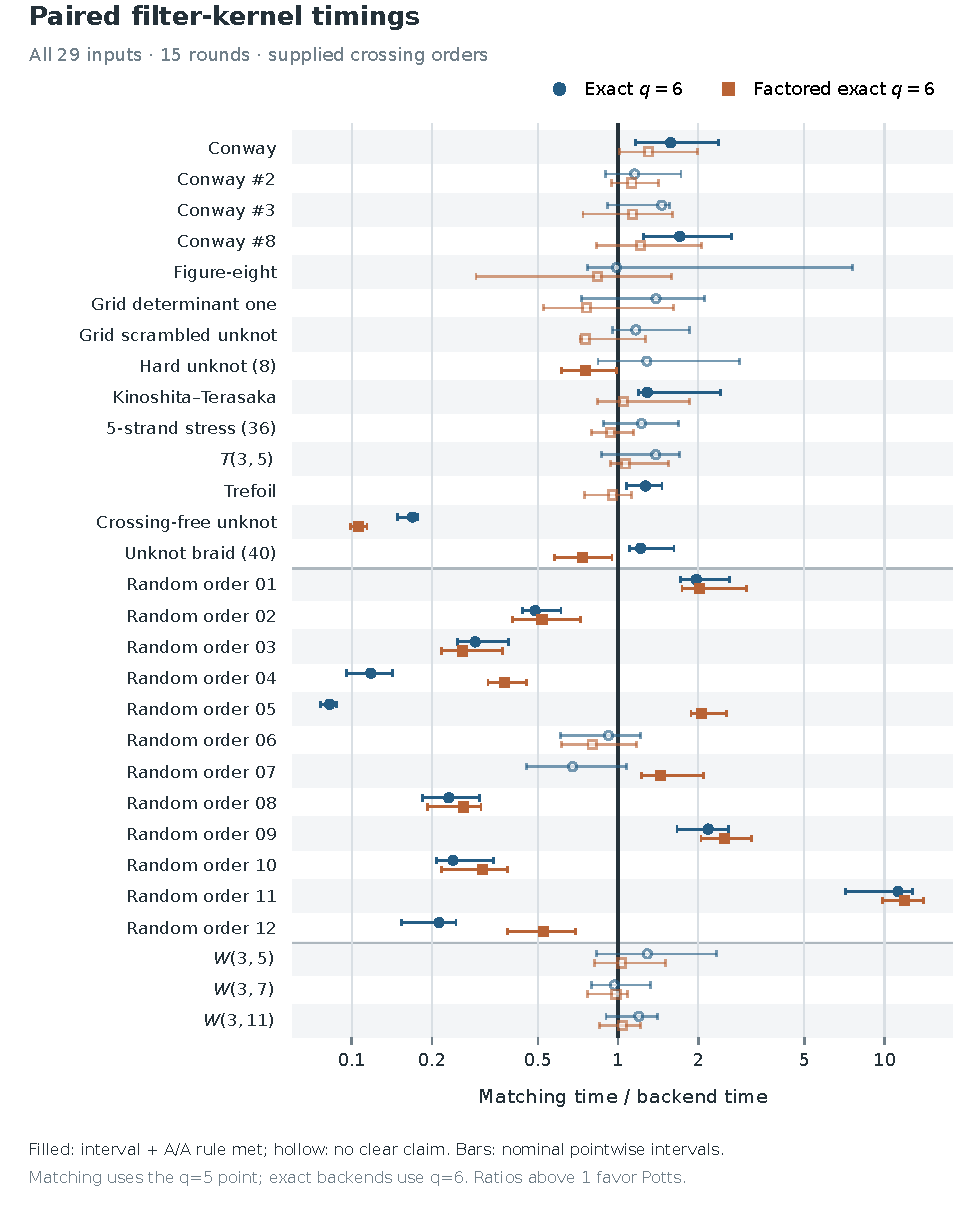
\includegraphics[width=\textwidth,height=0.87\textheight,keepaspectratio]{figures/kernel_ratios.pdf}
\caption{All 29 kernel comparisons against the same modular matching
reference. Ratios above one favor the indicated Potts arm. Exact $q=6$
uses a different Jones point from the modular reference. Intervals and
claim markers follow the recorded paired/A/A rule; regressions are shown
alongside improvements.}
\label{fig:ratios}
\end{figure}

\begin{figure}[htbp]
\centering
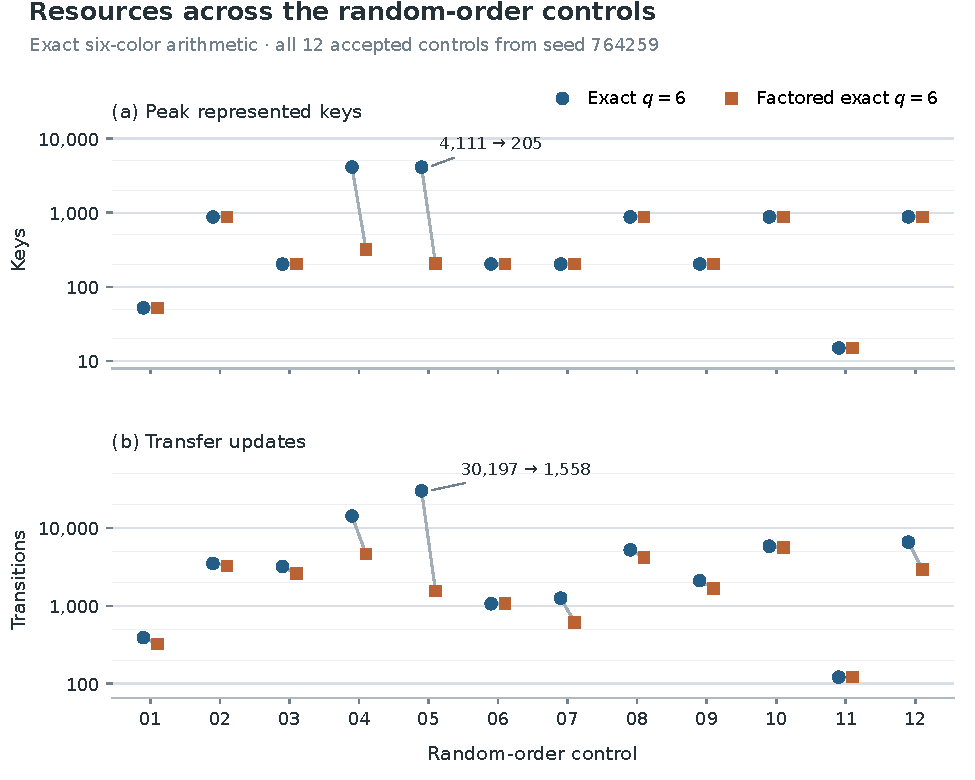
\includegraphics[width=\textwidth]{figures/component_resources.pdf}
\caption{Logical state and transition counts on all twelve fixed random-order
controls. These deterministic measures expose both the savings from
component independence and cases where little factorization is available.
State counts are not process-memory measurements.}
\label{fig:resources}
\end{figure}

Several larger named fixtures show favorable kernel medians, but many
intervals and A/A ranges are too wide to support a local claim for a
particular arm. These cases are retained without upgrading the evidence.
The examples establish that the representation can improve practical
work; they do not establish a growing-family runtime exponent.

\subsection{Normal-pipeline experiment}

A separate experiment contains \textbf{476 timed calls}: 17 inputs,
seven rotated rounds, matching A/A controls, exact $q=6$, and factored
exact $q=6$. It includes JSON parsing, validating diagram construction,
normal recognition and JSON output encoding. Imports, file I/O, CLI
parsing and process startup are excluded.
The matching backend uses its native generic $A$, and every ordinary
early stage remains enabled.

All verdicts are complete and consistent. Only five cases reach Jones:
Conway, Kinoshita--Terasaka, and Conway connected sums with two, three
and eight summands. The other twelve are decided earlier, including all
three weaving controls.

% Generated by make_paper_figures.py; do not edit values by hand.
\begin{table}[htbp]
\centering
\footnotesize
\setlength{\tabcolsep}{3.5pt}
\begin{tabular*}{\linewidth}{@{\extracolsep{\fill}}lrccc@{}}
\toprule
Input & $n$ & $T_M/T_E$ [interval] & $T_M/T_F$ [interval] & Supported claim \\
\midrule
Conway & 11 & 0.991 [0.448, 3.221] & 1.717 [0.605, 3.925] & None \\
Conway \#2 & 22 & 1.175 [0.582, 4.046] & 1.159 [0.286, 4.324] & None \\
Conway \#3 & 33 & 1.202 [0.292, 2.032] & 0.873 [0.426, 2.014] & None \\
Conway \#8 & 88 & 1.645 [0.474, 4.439] & 0.906 [0.346, 1.539] & None \\
Kinoshita--Terasaka & 11 & 1.374 [0.435, 3.422] & 1.973 [0.305, 3.946] & None \\
\bottomrule
\end{tabular*}
\par\smallskip
\begin{minipage}{\linewidth}\scriptsize
$M$: the normal pipeline with its native generic matching evaluation;
$E,F$: the normal pipeline with exact or factored exact $q=6$.
Nominal pointwise intervals; see the experimental-design assumptions in the text.
All five inputs reached Jones evaluation; the other twelve inputs bypassed it.
No comparison in this seven-round pipeline run met the timing-claim rule.
\end{minipage}
\caption{The five normal-pipeline cases that exercised the selected Jones backend. Timings include input parsing, checked diagram conversion, recognition, and JSON output encoding in a hot process.}
\label{tab:pipeline-selected}
\end{table}


\textbf{No full-pipeline speedup is supported by this seven-round run.}
The five cases that exercise Jones have wide intervals or A/A variation.
Backend speed claims are explicitly suppressed on bypassed cases.
This result limits the practical conclusion without weakening the proved
transfer bounds or the deterministic resource savings.

\subsection{Provenance and reproducibility limits}

The kernel source hashes agree before and after its timing run.
Subsequent edits changed only exact obstruction serialization wrappers and
added their shared helper; every raw evaluator and helper used in the
kernel timing has unchanged AST content. The exact measured versions of
all eight relevant modules were reconstructed and checked against the
recorded complete-file SHA-256 hashes. They are included as a provenance
snapshot, with the wrapper-only patch and audit record.
The normal-pipeline measurement uses the final wrappers and integrated
backends, with its own matching before/after hashes.

The corpus is small and timings are machine-dependent. Default budgets
were raised consistently for the kernel experiment to avoid comparing
early exits; all completed results and detection outcomes were checked.
There is no evidence here that a single representation dominates every
diagram, that an adaptive policy has already been validated, or that the
general recognizer has become quasi-polynomial.

\section{Residue characteristic polynomials and short algebraic certificates}
\label{sec:residue}

The Potts improvements act on a scalar obstruction. A separate line of
progress concerns the local rings that occur in exact categorical
Khovanov computation. Earlier ProveIt work already uses nilpotent radical
perturbations and finite geometric-series inverses
\cite{report08,report12}. The immediately preceding continuation constructs
Fitting decompositions of supplied \emph{scalar} binary endomorphisms.
We now extend the algebraic certificate mechanism to supplied ring-valued,
same-matching blocks.

The ingredients are standard Cayley--Hamilton, scalar Frobenius, polynomial
Chinese remainders, and Fitting decomposition. The theorem is stated with a
complete elementary proof because the applicable ring and matrix hypotheses
matter. This is not a literature-wide novelty claim about matrix nil indices.
No production scanner speedup from this supplemental result is claimed.

\subsection{A residue-only annihilator}

Fix a prime $p$ and positive integers $b,r$. Set
\[
 R_{b,p}=\F_p[x_1,\ldots,x_b]/(x_1^p,\ldots,x_b^p),\qquad
 J=(x_1,\ldots,x_b),\qquad B=b(p-1).
\]
Let $\rho:R_{b,p}\to\F_p$ take the constant coefficient.
The monomial basis has exponents $0\le\alpha_i<p$, so
$J^{B+1}=0$ and $J^B\ne0$. Scalar Frobenius gives
\begin{equation}
 a^p=\rho(a)\qquad(a\in R_{b,p}).
 \label{eq:scalar-frobenius}
\end{equation}
This identity concerns scalar elements of a commutative ring. The map
$A\mapsto A^p$ on matrices is not entrywise Frobenius and need not be additive.

\begin{theorem}[Residue characteristic-polynomial certificate]
\label{thm:residue}
For $A\in M_r(R_{b,p})$, put $A_0=\rho(A)$ entrywise and
$\chi_0(t)=\det(tI-A_0)\in\F_p[t]$. Then
\[
 \boxed{\chi_0(A)^p=0.}
\]
Thus $A$ has an explicitly computable annihilating polynomial
$\chi_0(t)^p$ of degree $pr$, independent of $b$.
\end{theorem}
\begin{proof}
Write $\chi_A(t)=\sum_{i=0}^r c_it^i$ over $R_{b,p}$, with $c_r=1$.
Taking constant coefficients commutes with the determinant, so
$\chi_0(t)=\sum_i\rho(c_i)t^i$.
Cayley--Hamilton over a commutative ring gives $\sum_i c_iA^i=0$.
These summands commute with each other: each is a scalar multiple of a
power of the same matrix. Consequently raising their sum to its $p$th power
is legitimate and yields
\[
 0=\sum_i c_i^p A^{pi}
   =\sum_i\rho(c_i)A^{pi}
   =(\chi_0(t)^p)(A)=\chi_0(A)^p.
\]
No Frobenius identity for arbitrary noncommuting matrix summands was used.
\end{proof}

The practical case here is $p=2$, where the dot algebra of a same-matching
block has square-zero variables. Its annihilator degree is at most $2r$,
even if the scalar coefficient space has dimension $2^b$.

\subsection{A sharp radical-matrix bound}

\begin{theorem}[Sharp universal radical cutoff]\label{thm:radical}
Every $N\in M_r(J)$ satisfies
\[
 N^L=0,\qquad L=\min\{b(p-1)+1,pr\}.
\]
For every $b,r\ge1$ and prime $p$, there is such an $N$ with
$N^{L-1}\ne0$.
\end{theorem}
\begin{proof}
The ideal bound gives $N^{B+1}=0$. Since $N_0=0$,
$\chi_0(t)=t^r$, and Theorem~\ref{thm:residue} gives $N^{pr}=0$.

For sharpness, let $s=\min(b,r)$. Use an $s\times s$ upper-bidiagonal block
with distinct variables $x_1,\ldots,x_s$ on the diagonal. Of its $s-1$
superdiagonal positions, label
\[
 e=\min\{s-1,(b-s)(p-1)\}
\]
with variables among $x_{s+1},\ldots,x_b$, each used at most $p-1$ times.
Label the remaining positions with diagonal variables, again with each
used at most $p-1$ times. There is enough capacity since
$s-1\le s(p-1)$. Let $a_i$ be the number of superdiagonal entries labeled
$x_i$ for $i\le s$.

In a power of this bidiagonal matrix, a path from row $1$ to column $s$
traverses every superdiagonal position in its forced order and can wait
at vertex $i$ by using the diagonal $x_i$. Choose exactly $p-1-a_i$ waits
at that vertex. The resulting monomial has degree
\[
 D=(s-1)+\sum_{i=1}^s(p-1-a_i)
  =s(p-1)+e
  =\min\{b(p-1),pr-1\}=L-1.
\]
Every variable exponent is below $p$. Its coefficient is one: the
superdiagonal order is forced and the distinct diagonal variables specify
the waiting counts uniquely. Hence it survives in the $(1,s)$ entry of
$N^D$. Embed the block into an $r\times r$ zero matrix when $s<r$.
\end{proof}

For $p=2$ the cutoff is $\min(b+1,2r)$.
When $b\ge2r-1$, a particularly transparent witness has $r$ distinct
diagonal variables and $r-1$ further distinct superdiagonal variables.
The $(1,r)$ entry of $N^{2r-1}$ is their product.
This shows that replacing $2r$ by $r$, based on a scalar square-zero
intuition, would be wrong.

If instead $A_0$ is nilpotent of index $s$, then $A^s\in M_r(J)$.
Combining the ideal bound with Theorem~\ref{thm:residue} yields
\begin{equation}
 A^{\min\{pr,\ s[b(p-1)+1]\}}=0.
 \label{eq:nilpotent-residue}
\end{equation}
The $pr$ term can be attained already with one variable: the companion
matrix of $t^r-x_1$ has $A^r=x_1I$ and nilpotence index $pr$.
We do not claim simultaneous sharpness of \eqref{eq:nilpotent-residue}
for every prescribed triple $(b,r,s)$.

\subsection{Inverses without a determinant over the large ring}

\begin{corollary}\label{cor:inverse}
For $N\in M_r(J)$,
\[
 (I+N)^{-1}=\sum_{j=0}^{L-1}(-N)^j,\qquad
 L=\min\{b(p-1)+1,pr\}.
\]
More generally, if $A_0$ is invertible and
$\chi_0(t)=\sum_{i=0}^r c_it^i$, then
\[
 A^{-1}=-c_0^{-1}\sum_{i=1}^r c_iA^{pi-1}.
\]
\end{corollary}
\begin{proof}
The first formula telescopes using $N^L=0$.
For the second, Theorem~\ref{thm:residue} says
$c_0I+\sum_{i=1}^r c_iA^{pi}=0$.
Multiplying the proposed inverse on either side by $A$ gives $I$.
\end{proof}

At $p=2$, the minus signs disappear and $c_0=1$.
The characteristic polynomial is computed over the small base field, not
by expanding a determinant with $2^b$ coefficients in each entry.
The powers of $A$ still require actual ring arithmetic.
If a geometric series is evaluated by doubling a power-and-partial-sum
pair, it takes $O(\log L)$ matrix products. The comparison with earlier
methods must acknowledge this: reducing a cutoff from $b+1$ to $2r$
does not automatically save $b/r$ matrix products in an already doubled
implementation.

\subsection{Constructive Fitting and Drazin data}

Factor the residue characteristic polynomial as
\[
 \chi_0(t)=t^a q_0(t),\qquad q_0(0)\ne0.
\]
The notation $q_0$ here is a polynomial and is unrelated to a Potts color
count. Polynomial CRT gives a residue class $e(t)$ modulo
$t^{pa}q_0(t)^p$ satisfying
\[
 e(t)\equiv0\pmod{t^{pa}},\qquad
 e(t)\equiv1\pmod{q_0(t)^p}.
\]
Choose its representative of degree below $pr$ and set $E=e(A)$.

\begin{theorem}[Explicit Fitting projectors]\label{thm:fitting}
The operators above satisfy
\[
 E^2=E,\quad AE=EA,\quad A^{pa}(I-E)=0,\quad q_0(A)^pE=0.
\]
There is a polynomially specified $D$ with
$AD=DA=E$ and $DE=ED=D$.
The modules $\ker E$ and $\im E$ are free of ranks $a$ and $r-a$,
and a concrete basis change can be lifted from residue projector columns.
\end{theorem}
\begin{proof}
All displayed identities for $E$ follow from polynomial divisibility by
$t^{pa}q_0^p$ and Theorem~\ref{thm:residue}.
Choose $z(t)$ by CRT with $z=0$ modulo $t^{pa}$ and
$z=t^{-1}$ modulo $q_0^p$, and let $D=z(A)$.
The claimed identities follow by the same argument.
In particular $A$ is nilpotent on $\ker E$ and invertible on $\im E$.
The limiting cases $a=0$ and $a=r$ use $E=I$ and $E=0$ respectively.

Choose columns of $E_0$ spanning $\im E_0$ over $\F_p$, and columns of
$I-E_0$ spanning $\ker E_0$. Take the corresponding columns of $E$ and
$I-E$ and arrange the kernel columns first in a matrix $P$.
Its residue $P_0$ is invertible. Since $R_{b,p}$ is local with maximal
ideal $J$, $\det P$ is a unit, so $P$ is invertible.
The column identities give
$EP=P\operatorname{diag}(0_a,I_{r-a})$, proving the rank and basis claims.
\end{proof}

The resulting $D$ is the Fitting/Drazin inverse:
$DAD=D$ and $A^{pa+1}D=A^{pa}$.
The method constructs the decomposition inside matrices over $R_{b,p}$.
It need not first expand the module to dimension $rp^b$ over the base field.
It nevertheless must represent and manipulate its ring coefficients.

\subsection{Intertwining across categorical blocks}

Suppose a finite additive $\F_p$-linear category contains same-matching
objects $X_i$ with $\End(X_i)=R_{b_i,p}$, and a degree-preserving chain
endomorphism $Q$ is block diagonal by degree and matching.
Write $A_i$ for its block on $X_i^{r_i}$. A differential component $T$
satisfies $A_jT=TA_i$ under actual categorical composition.

Construct the respective $E_i,D_i$ and $E_j,D_j$ by the preceding theorem.
Their projector polynomials need not be the same.
For $N$ large enough to kill both nilpotent restrictions,
\[
 (I-E_j)TE_i
  =(I-E_j)TA_i^ND_i^N
  =(I-E_j)A_j^NTD_i^N=0.
\]
Similarly,
\[
 E_jT(I-E_i)
  =D_j^NA_j^NT(I-E_i)
  =D_j^NTA_i^N(I-E_i)=0.
\]
Hence $E_jT=TE_i$, and the nilpotent and invertible images form
complementary subcomplexes. The lifted bases exhibit a genuine chain
isomorphism when every inverse and categorical cross term is evaluated.

The characteristic-polynomial theorem is used only inside the commutative
same-matching endomorphism blocks. Applying it directly to an arbitrary
mixed-matching matrix with noncommutative cobordism entries would be invalid.
Finding useful $Q$, keeping it small, and exploiting the resulting summands
are separate algorithmic problems.

\subsection{How this advances the previous continuation}

The previous scalar Fitting procedure already stabilizes in at most its
matrix dimension over $\F_2$. The $2r$ annihilator does not accelerate that
scalar computation. Its contribution is a ring-valued certificate whose
polynomial degree is controlled by block multiplicity rather than only by
the number of dot variables. The sharpness theorem prevents an unjustified
further truncation.

The supplied oracle represents monomials by exponent tuples and checks the
identities independently of the production dot algebra. Its characteristic
polynomial routines are intended for small exhaustive experiments, not as a
scalable implementation. The exact counts are reported in
Section~\ref{sec:experiments}. No bound on all scanner multiplicities,
all block sizes, or closure of a succinct representation follows from
these local theorems.

\section{The remaining distance to quasi-polynomial recognition}
\label{sec:complexity}

\subsection{Three separate obstacles}

A faster exact scalar filter addresses only one part of the recognition
problem. Three distinct missing implications must not be conflated.

First, equality of a selected Jones value to $1$ need not decide the knot.
At $q=5$ this is disproved by Theorem~\ref{thm:blind}; at $q=6$ we assume
no global detection statement. The completeness of the enclosing recognizer
comes from its retained exact fallback, not from these evaluations.

Second, the input diagram does not come with a promise of logarithmic or
polylogarithmic width. Theorems~\ref{thm:transfer} and
\ref{thm:componentwidth} are bounds in a supplied order's measured
parameters. A polynomial heuristic finds useful orders but has no universal
$O((\log n)^2)$ guarantee. Planar separator methods and tensor contraction
are relevant, established tools \cite{maria2021,seymour1994}; using them does
not imply a polylogarithmic bound for arbitrary diagrams.

Third, the full categorical complex contains more information than the
scalar partition function. Boundary size does not alone control object
multiplicities, ranks, differential supports or the size of an explicit
homology basis. Kelomäki and Schütz prove exponential behavior for explicit
scanning or divide-and-conquer constructions even on certain positive and
alternating three-braid families, while giving polynomial algorithms for
compressed three-braid homology and fixed homological windows at fixed strand
count \cite{kelomaki2026}. This is a representation obstruction, not a reason
to abandon compression.

\subsection{A finite exact menu decides Jones-polynomial triviality}

The fixed-color obstruction can be extended to an unconditional decision
about the entire Jones polynomial, although this still does not settle
unknot recognition.

\begin{proposition}[A growing exact specialization menu]\label{prop:menu}
For a knot diagram with $n>0$ crossings, suppose the exact quadratic
evaluations equal $1$ for every integer
$q\in\{5,6,\ldots,2n+5\}$. Then $V_D(t)$ is identically $1$.
Conversely, the constant polynomial $1$ passes every evaluation.
On a supplied order of width $w$, this decision can be carried out using
the one-tensor algorithm in
\[
 n^{\lfloor w/2\rfloor+O(1)}
\]
bit operations. In particular it is quasi-polynomial when
$w=O(\log n)$.
\end{proposition}
\begin{proof}
In a normalized smoothing summand, the $A$ exponents come from a smoothing
weight in $[-n,n]$, the writhe correction in $[-3n,3n]$, and
$\delta^{c-1}$ with $c-1\le n$. Hence all $A$ exponents lie in $[-6n,6n]$.
For a knot they are multiples of four, so all Jones $t$ exponents lie in
the conservative interval $[-2n,2n]$.
Thus $P(t)=t^{2n}(V_D(t)-1)$ is a polynomial of degree at most $4n$.

Equality at a root of $t^2-(q-2)t+1$ makes this irreducible quadratic divide
$P$ over $\Q$. The $2n+1$ quadratics for the specified distinct values of
$q$ are pairwise coprime. If $P\ne0$, their product of degree $4n+2$
cannot divide it. Thus $P=0$.

There are $O(n)$ evaluations with $q=O(n)$. For $f\le w/2\le n$,
the number of equality patterns is at most the Bell number
$B(f)\le f^f\le n^f$, with the empty pattern treated separately.
Introducing two vertices has only $O((f+2)^2)$ canonical branches,
independent of the multiplicities attached to those branches.
The coordinate lengths are $O(n\log n)$ by Theorem~\ref{thm:bits}.
All remaining factors, including exact arithmetic and normalization, are
polynomial in $n$ and $w$.
\end{proof}

A smaller menu follows from the same proof without new topology.
For writhe $r$, the actual conservative exponent interval is
$[\lceil3(r-n)/4\rceil,\lfloor3(r+n)/4\rfloor]$.
It contains zero and has width $D\le\lfloor3n/2\rfloor$.
Thus $\lfloor D/2\rfloor+1$ distinct quadratic evaluations suffice.
The larger $2n+1$ menu keeps the statement independent of this refinement.

This is elementary degree counting, not a new claim about the difficulty of
the Jones polynomial. It shows exactly what a sufficiently large menu can
certify. The menu is a mathematical extension; the default recognizer does
not automatically run $O(n)$ different color counts. The complete
unknot-detection question for $V_D(t)\equiv1$ remains outside its conclusion.
It also shows why a growing number of colors cannot be hidden in a
fixed-$q$ complexity statement.

\subsection{A precise conditional algebraic route}

Reduced Khovanov rank one characterizes the unknot
\cite{kronheimer2011}. The same rank-one decision is sound over $\F_2$:
rank one over $\F_2$ forces rational rank at most one by universal
coefficients, while reduced knot homology is nonzero; the rational
rank-one theorem then applies. Conversely the unknot has reduced rank one
over $\F_2$.
The baseline's local-complex and cancellation approach follows the practical
framework of Bar-Natan~\cite{barnatan2007}; a general small-complex bound
is a separate requirement.

To turn that endpoint into a quasi-polynomial algorithm, a compression
scheme needs a closed set of operations and a size theorem, not merely
small examples or an existence statement.

\begin{theorem}[Conditional summary criterion]\label{thm:conditional}
Let $Q(n)=\exp((\log(n+2))^c)$ for a fixed constant $c$.
Suppose a proposed exact recognition method has, on every $n$-crossing
input, the following proved properties:
\begin{enumerate}
\item it constructs at most $Q(n)$ summaries or intermediate states;
\item each summary has at most $Q(n)$ bits;
\item constructing, composing, restricting, simplifying, comparing, and
checking a summary uses at most $Q(n)^{O(1)}$ bit operations;
\item a final predicate, evaluable within the same bound, is equivalent to
reduced Khovanov rank one or to another complete unknot criterion.
\end{enumerate}
Then the resulting exact recognizer is quasi-polynomial time.
\end{theorem}
\begin{proof}
Multiply the number of operations by their cost. A fixed power of
$\exp((\log(n+2))^c)$ is still quasi-polynomial. Exact invariants and the
terminal equivalence imply correctness.
\end{proof}

The theorem is intentionally a contract rather than a breakthrough: its
hypotheses identify the work still missing. The Potts representations satisfy
analogous storage and operation bounds at bounded width, but their terminal
predicate is incomplete. The residue-polynomial theorem shortens a local
certificate, but does not prove the global summary count or size. The earlier
scalar splitter finds some endomorphisms but does not guarantee a useful
decomposition on every input.

For an explicit ring-valued implementation, the coefficient space alone has
$p^b$ basis monomials. A block with multiplicity $r$ can have $r^2$
entries. Bounding an inverse polynomial's degree by $pr$ leaves both
$p^b$ and the total number of blocks to be controlled.
Using a circuit or shared DAG can reduce their representation, but then
composition, equality and zero detection for that representation also require
proved bounds. Constant-size formulas whose expansion is exponential do not
by themselves satisfy the criterion.

\subsection{The geometric route and the current literature}

Lackenby's 2021 slides announce a deterministic recognition algorithm with
bound $2^{O((\log n)^3)}=n^{O((\log n)^2)}$ \cite{lackenby2021}.
That is quasi-polynomial, but it is not the stronger
$n^{O(\log n)}$ target sometimes used in project notes.
The July 2026 hierarchy preprint supplies a new recognition algorithm and
certification framework; its Section 9 separates iteration counting from
the cost of operations and bounds iterations by $L(G+1)^L$,
where $L$ is maximum hierarchy length and $G$ maximum surface
pattern-complexity \cite{lackenby2026}. We use $G$ here to distinguish it
from the component frontier $g$.

Published compressed-curve algorithms compute intersection numbers with
cost polynomial in triangulation size and logarithmic normal weights;
the isotopy result additionally assumes essential normal one-manifolds
\cite{lackenbycurves2026}. These provide concrete components for a geometric
implementation. Neither a fast terminal-pattern check nor an iteration
count by itself supplies a complete bound on construction, cutting,
simplification, representation growth and restarts.

For example, an independently proved bound $L=O(\log n)$ and
$G=n^{O(1)}$ would make $L(G+1)^L=n^{O(\log n)}$; with
$L=O((\log n)^2)$ it would give $n^{O((\log n)^2)}$.
These are conditional substitutions, not bounds established for the
hierarchy inputs generated by this package. Likewise, a bit cost polynomial
in an expanded normal weight is inadequate when that weight is exponential
in its encoded length.

The strongest credible program therefore has two interacting branches:
exact algebraic obstructions and compressed homological decisions for
efficient practical rejection, and fully costed compressed geometric
operations for a possible general recognition guarantee. They should share
validated inputs, deterministic evidence records and resource-safe
orchestration, while retaining separate mathematical obligations.

\section{Further research questions and concrete next experiments}
\label{sec:research}

The following program distinguishes short implementation projects,
structural mathematical questions, and obligations needed for a full
complexity theorem. A successful next step should produce either a proof
with explicit hypotheses, an independently replayable improvement, or an
informative counterexample.

\subsection{Immediate work on scalar transfers}

\begin{question}[Optimize the actual component cost]\label{q:order}
Can crossing orders and checkerboard colors be chosen to minimize merge
work, rather than only the global cut-edge or active-face maximum?
\end{question}

The current shading heuristic minimizes $(\max f_i,\sum f_i)$, while
Theorem~\ref{thm:componentwidth} depends on $g$ and actual work also depends
on alignment counts. A useful objective combines the sum of component orbit
counts, the products at merge steps, and estimated integer lengths.
Compute these structural features without running the full tensor
contraction, then compare greedy local changes on a fixed corpus.
The benchmark should include construction time and preserve orders on which
the existing heuristic wins. A worst-case approximation guarantee for this
objective would be more valuable than a favorable average alone.

\begin{question}[Switch representations at justified points]
Can a certified runtime policy choose among matching, one-tensor Potts,
and component Potts without paying their full combined costs?
\end{question}

The present measurements disprove a universal dominance claim. A first
policy can select an algorithm from cheap structural profiles and give each
attempt a fixed work budget. A stronger policy would convert a partially
computed representation when its cost grows. Such a conversion needs an
explicit linear map and an exact normalization account. Training a heuristic
on these 29 examples and reporting its accuracy on the same examples would
not answer the question; use held-out diagrams and relabeling controls.

\begin{question}[Factor beyond processed connected components]
When can an exact active tensor be split along articulation vertices,
small separators, or algebraic low-rank structure?
\end{question}

Graph-component independence is sufficient but not necessary for a compact
tensor. At a one-vertex separator, condition on the separator spin and
exploit the remaining color stabilizer. At larger separators, equality
patterns induce different stabilizer groups and orbit multiplicities.
The first milestone is a complete merge-and-forget calculus for separators
of size one and two, checked against labeled enumeration.
Algebraic rank factorization must preserve signed exact coefficients and
must charge for rank discovery. A large output rank supplies a natural
counterexample to an overly broad compression conjecture.

\begin{question}[Use contraction trees without assuming disk frontiers]
Can a tree-based exact Potts contraction improve path-order bottlenecks in
the repository while retaining the symmetry quotient?
\end{question}

Existing tensor and graph-width literature provides the starting point
\cite{meichanetzidis2019,maria2021}. The implementation question is how to
combine separator assignments, spin orbits and exact coefficient growth in
a reproducible cost model. A contraction tree should be stored as part of
the computation input and validated. Compare total contractions, maximum
tensor size, integer lengths and order-search cost. A tree decomposition
is useful only if its conversion and join operations are also bounded.

\subsection{Detection strength and exact specializations}

\begin{question}[Characterize the kernel of the six-color evaluation]
Which nontrivial knots, if any, have $V_K(2+\sqrt3)=1$?
\end{question}

This is a structural question about a specific evaluation. Start with
families having exact trace or skein recurrences: closed braids of fixed
index, twist constructions, satellites with controlled pattern, and
connected sums. Search for polynomial divisibility by $t^2-4t+1$ using
exact Laurent polynomials. A found collision is valuable even if another
filter already detects the knot. Failure to find one in a knot table gives
no completeness theorem.

\begin{question}[Design a small complementary menu]
Can a bounded or slowly growing set of algebraic points eliminate broad
classes of collisions while keeping total work small?
\end{question}

The $q=5$ failure and $q=6$ repair show why algebraic complementarity matters.
Measure additional detections per unit of exact work, with first-passing
and never-detected cases recorded. Distinguish changing $q$ from changing a
prime at fixed $q$. Proposition~\ref{prop:menu} gives an unconditional
growing menu for detecting whether the full Jones polynomial is $1$;
improving its number of points on a proved class is a concrete target.
A universal fixed menu would require a new theorem about the possible
Jones polynomials of knots.

\begin{question}[Arithmetic circuits or reconstruction]
Can modular evaluation and certified reconstruction outperform integer
pairs for very long, narrow diagrams?
\end{question}

The exact bit bound supplies an a priori reconstruction threshold.
One could evaluate over enough compatible primes, reconstruct each
coordinate, and verify with an additional exact identity. It is essential
to count prime selection, conversions, and total bit work. Pair arithmetic
has unusually cheap local multipliers, so a modular strategy may lose on
moderate inputs. Large-parameter tests should use the same diagram order
and report integer sizes, not merely crossing count.

\begin{question}[Shorter certificates than full replay]
Can a nontrivial exact Potts value be certified with a verifier materially
faster than recomputing the transfer?
\end{question}

The current evidence stores inputs and exact outputs, so replay has the
same complexity class as evaluation. A contraction transcript can expose
local sums and products, but may be as large as the computation.
Explore checkable arithmetic circuits, deterministic residual identities,
or interactive-verification models with their assumptions stated.
A soundness claim must account for arbitrary forged intermediate tables,
not just altered final values.

\subsection{Ring-valued compression for the complete fallback}

\begin{question}[Find useful ring-valued chain endomorphisms]
Can the scalar candidate search from the preceding continuation be extended
to produce small nontrivial same-matching ring-valued endomorphisms?
\end{question}

Theorem~\ref{thm:fitting} assumes the operator is supplied. A concrete
experiment is to add low dot-degree unknowns to the scalar intertwining
equations, solve them exactly, and test whether the lifted Fitting summands
reduce work on actual scanner blocks. Record the search dimension, solution
support, block sizes before and after splitting, and the cost of checking
all categorical cross terms. A search that routinely costs more than the
saved elimination is not a performance improvement.

\begin{question}[Exploit low annihilator degree]
When is the residue characteristic polynomial substantially larger than a
usable annihilator, and can a shorter one be found cheaply?
\end{question}

The universal certificate has degree $pr$, and the radical cutoff is sharp
in the full class. Particular matrices may have much smaller residue
minimal polynomials or additional relations. A residue minimal polynomial
alone need not lift with exponent $p$ by the proof of
Theorem~\ref{thm:residue}; that proof uses characteristic-polynomial
coefficients over the large ring. The first task is to identify a valid
lifting theorem or an explicit counterexample before replacing the
characteristic polynomial in code. Compare any successful refinement with
doubled geometric-series inversion.

\begin{question}[Keep Fitting projectors succinct]
Can $e(A)$ and its basis changes be manipulated without expanding their
coefficient supports or multiplicity spaces?
\end{question}

A degree-$O(r)$ polynomial is short, but evaluating it can create large
entries. Candidate representations include sparse monomial maps, shared
composition DAGs, and block recurrences. Each needs exact addition,
composition, zero testing, and application to differentials. The target
is a closure theorem bounding all these operations on a specified class.
Measure both the representation size and the cost of operations performed
on it; a small serialized expression can still hide expensive evaluation.

\begin{question}[Decision information without full homology]
Which exact summaries retain the rank-one question under all tangle
extensions while discarding irrelevant homology?
\end{question}

Previous saturated decisions and homological windows suggest useful
restricted summaries, but a complete invariant of future continuations can
be much larger than a scalar Euler characteristic. Formulate a congruence
on partial complexes that is respected by every allowed crossing extension.
Prove that the terminal decision descends to the quotient. Then either
bound the number of quotient states or exhibit a family requiring many.
This is a direct route toward the missing hypotheses of
Theorem~\ref{thm:conditional}.

\begin{question}[Learn from the explicit three-braid barrier]
Which features permit compressed three-braid algorithms, and which survive
at four or more strands?
\end{question}

The 2026 results provide both a warning about explicit output size and a
positive compressed model \cite{kelomaki2026}. A useful next project is to
encode a proven fixed-strand family with exact multiplicities and verify
the closed recurrences against the baseline scanner.
The research target is an extension theorem with a precise parameter,
not an empirical claim that all fixed-width complexes remain small.

\subsection{A fully costed geometric branch}

\begin{question}[Implement compressed normal-curve operations]
Can the published intersection and isotopy algorithms be integrated with
ProveIt's boundary-pattern representation?
\end{question}

The initial deliverable should handle explicit triangulated surfaces,
binary normal coordinates, geometric intersection numbers and the essential
curve precondition for isotopy \cite{lackenbycurves2026}.
Tests must include exponentially large weights described by short binary
inputs. Enumerating all normal arcs would destroy the intended complexity.
Every conversion between patterns, triangulations and normal coordinates
must be part of the time and size account.

\begin{question}[Control hierarchy restarts and encodings]
What invariant gives a useful simultaneous bound on hierarchy length,
pattern complexity, representation size and restart cost?
\end{question}

The expression $L(G+1)^L$ motivates a quantitative target but is not itself
a complete running-time theorem. Instrument an implementation of one
well-defined hierarchy step and prove that its compressed output meets a
stated bound. Then analyze how cutting and simplification interact with
that bound under restarts. A fast terminal checker is already a useful
component; the next milestone is a fully costed nonterminal transition,
followed by a global potential argument.

\begin{question}[Connect the algebraic and geometric branches]
Can an exact algebraic obstruction or partial homological summary guide
geometric choices without becoming an unproved pruning rule?
\end{question}

A safe interaction uses algebraic information to prioritize work while
retaining every branch required by the geometric correctness proof.
A stronger pruning rule needs its own implication theorem.
The first practical milestone is shared diagram and certificate formats
with explicit preprocessing equivalences. The longer-term milestone is
a combined algorithm whose worst-case bound can be proved independently
of its heuristic ordering choices.

\subsection{Evaluation discipline and recommended sequence}

Before a broad default change, extend the corpus beyond small named
fixtures and short random braids. Include pairs of diagrams of the same
knot with different embeddings and orders, nontrivial Alexander-trivial
knots, difficult unknot diagrams, large connected sums, and families chosen
to stress each representation. Record cases solved before the Jones stage
separately. Measure failed or budget-limited attempts as costs, not as
missing data.

The recommended sequence is: first improve the component-aware order
objective and confirm it on held-out inputs; next extract actual
same-matching blocks to test the residue certificates; then implement one
compressed geometric operation with a complete bit-complexity contract.
In parallel, maintain the exact-specialization collision search and the
independent oracles. This sequence produces useful verified increments
while keeping the eventual quasi-polynomial theorem tied to explicit,
testable obligations.

\section{Reproducibility, integration, and the final research position}
\label{sec:reproduction}

\subsection{Contents of the archive}

\begin{longtable}{@{}p{0.27\textwidth}p{0.67\textwidth}@{}}
\toprule
Location & Contents\\
\midrule
\endfirsthead
\toprule Location & Contents\\ \midrule
\endhead
\code{paper/} &
This PDF, the main LaTeX source, all section sources, BibTeX references,
generated tables, vector figures and preview PNGs.\\
\code{fast/} &
The modified implementation, all existing fixtures and tests, four Potts
modules, integration tests and the new backend guide.\\
\code{reference/} &
The selected pinned repository snapshot, including the baseline
implementation and research notes used for the audit.\\
\code{integration/} &
The patch against the pinned tree, a list of changed files, source
provenance and Git blob identifiers.\\
\code{research/} &
Independent smoothing-cube, finite-menu and truncated-ring oracles;
proof-audit notes; certificate replayer; saved verification records and
baseline/modified test logs.\\
\code{benchmarks/} &
Kernel and normal-pipeline scripts, all raw samples, CSV summaries,
source-hash audits, measured module versions and figure-generation code.\\
\code{certificates/} &
Example exact $q=6$ obstruction certificates, the $W_5$ collision record,
and saved replay results.\\
\code{tools/} &
Manifest and patch verification, certificate regeneration, and a
reproduction driver that writes to a fresh run directory.\\
\code{SHA256SUMS} &
SHA-256 digest list for distributed files.\\
\bottomrule
\end{longtable}

The source snapshot contains 98 selected text files whose Git blob hashes
were checked at retrieval. It is not represented as a complete clone of the
entire ProveIt repository. The integration patch affects only the
\code{Topology/UnknotRecognition/fast/} subtree.
It adds the new modules and tests, changes the Jones dispatch and CLI budget
handling, and documents the options. It leaves the categorical fallback
implementations intact.

\subsection{Reproducing the mathematical and software checks}

From the root of the extracted archive:
\begin{lstlisting}
python tools/verify_manifest.py
python tools/verify_integration.py
python tools/reproduce.py
\end{lstlisting}
The manifest checker verifies both archive digests and pinned Git object
hashes. The integration checker applies the patch to a disposable copy and
compares the resulting source bytes with the delivered implementation.
The reproduction driver runs the integrated unit suite, independent
oracles, replay self-tests and supplied certificates in a new directory.
It preserves the distributed result records and writes commands, durations,
exit codes and logs for the new run.

To repeat the timings, the large-integer check and the PDF build as well:
\begin{lstlisting}
python tools/reproduce.py --all
\end{lstlisting}
Timing outputs should not be expected to match the distributed nanosecond
samples. Exact values, deterministic work counters, test results and
certificate verdicts should match. Differences in Python version,
machine load and platform are recorded by the scripts.

Core algorithms and validation use the Python standard library.
The implementation requires Python 3.10 or later; the recorded environment
used 3.12.14. Regenerating the figures requires Matplotlib.
The paper uses pdflatex, BibTeX, latexmk and the packages listed in its
preamble. The complete source is included so that layout, notation,
references and integration conventions can be revised in the repository.

The independent oracles are intentionally small-instance tools.
The smoothing cube is exponential in crossing number. The truncated-ring
oracle uses explicit monomials and small matrix characteristic polynomials.
They test the optimized algorithms through a different representation;
they are not proposed as scalable alternatives.

\subsection{Integration procedure}

At a checkout of the pinned ProveIt revision, run:
\begin{lstlisting}
git apply --check /path/to/package/integration/changes.patch
git apply /path/to/package/integration/changes.patch
\end{lstlisting}
The patch has been checked by applying it to the included reference copy
and comparing all resulting implementation files. A later repository
revision may require an ordinary merge. The article and its associated
research artifacts can be placed in a new report directory using the
project's preferred numbering.

The package retains the source's MIT No Attribution license and supplies
the continuation code and documentation under the same license.
Scholarly sources are cited through their primary papers and author or
publisher pages; the archive does not redistribute copies of those papers.
This is a mathematical research draft with reproducible experiments,
not a proof-assistant formalization.

\subsection{What the continuation establishes}

There is a concrete, verified scalar improvement: fixed-color equality
patterns and component independence give a smaller, precisely bounded
representation for a Jones obstruction. Exact quadratic arithmetic makes
its bit cost and equality semantics explicit. The five-color weaving family
shows why exact arithmetic alone is insufficient, while the six-color
calculation gives a proved repair of that family. The growing menu gives a
separate quasi-polynomial Jones-triviality decision on logarithmic-width
orders.

There is also a precise local algebraic advance: residue characteristic
polynomials give bounded-degree annihilators, sharp radical cutoffs and
constructive Fitting certificates for supplied commutative endomorphism
blocks. These results extend the available tools without assuming that the
entire categorical computation remains small.

The next general recognition theorem must still connect an exact complete
criterion to a globally bounded representation and a fully costed search.
The archive is intended to make the present increments usable while keeping
that larger obligation visible and mathematically testable.

\clearpage
\begingroup
\raggedright
\small
\bibliographystyle{plainnat}
\bibliography{references}
\endgroup
\end{document}
